\documentclass[10pt]{beamer}

\newcommand\hmmax{0}
\newcommand\bmmax{0}
\usetheme[subsectionpage=progressbar]{metropolis}
\setbeamertemplate{section in toc}[sections numbered]
\setbeamertemplate{subsection in toc}[circle]
\setbeamerfont{subsection in toc}{size=\small}
\usepackage{algorithm}
%\usepackage{subcaption}
\usepackage{xargs}
\usepackage{algorithmic,algorithm}
\usepackage{appendixnumberbeamer}
\usepackage[authoryear,round]{natbib}
\usepackage{booktabs}
\usepackage{mdframed}
\newmdtheoremenv{theo}{Theorem}
\newmdtheoremenv{prop}{Proposition}
\newmdtheoremenv{lem}{Lemma}
\newmdtheoremenv[
  bottomline=true,
  topline=true,
  rightline=true,
  leftline=true]{lemm}{Lemma}
\newmdtheoremenv{coro}{Corollary}
\usepackage[scale=2]{ccicons}
\usepackage{tikz}
\usetikzlibrary{positioning}
\usepackage{pgfplots}
\usepgfplotslibrary{dateplot}
\setbeamertemplate{theorems}[numbered]
\setbeamertemplate{section in toc}{\inserttocsectionnumber.~\inserttocsection}
\usepackage{xspace}
\usepackage{stmaryrd} 
\usepackage{mathtools} 
\usepackage{amsmath,amssymb,amsthm,mathrsfs}
\usepackage{multicol}
\newcommand{\KLD}[2]{\mathrm{KL} \left( \left. \left. #1 \right|\right| #2 \right) }
\newcommand{\themename}{\textbf{\textsc{metropolis}}\xspace}
\newcommand{\map}{\hat{\psi}_i}
\newcommand{\phimap}{\hat{\phi}_i}
\newcommand{\expec}{\mathbb{E}}
\newcommand{\logl}{\texttt{L}}
\newcommandx\sequence[3][2=,3=]
{\ifthenelse{\equal{#3}{}}{\ensuremath{\{ #1_{#2}\}}}{\ensuremath{\{ #1_{#2}, \eqsp #2 \in #3 \}}}}
\newcommandx\sequencePar[3][2=,3=]
{\ifthenelse{\equal{#3}{}}{\ensuremath{\{ #1({#2})\}}}{\ensuremath{\{ #1({#2}), \eqsp #2 \in #3 \}}}}

\newenvironment{variableblock}[3]{%
  \setbeamercolor{block body}{#2}
  \setbeamercolor{block title}{#3}
  \begin{block}{#1}}{\end{block}}
\newcommand{\dens}{\texttt{p}}
\definecolor{myblue}{HTML}{4b7cf1}
\definecolor{myblack}{HTML}{000000}
\definecolor{mywhite}{HTML}{ffffff}
\setbeamercolor{frametitle}{fg = myblue,bg=mywhite}
\setbeamercolor{normal text}{fg=myblack, bg = mywhite}
\setbeamerfont{frametitle}{size=\fontsize{16}{43.2}}              
\newcommand{\trans}[1]{#1^\prime}
\def\thml{\hat{\theta}_{\rm ML}}
 \newtheorem{Fact}{Fact}
\newtheorem{Prop}{Proposition}
\newtheorem{Def}{Definition}
\newtheorem{Property}{Property}
\newtheorem{Observation}{Observation}
%\theorembodyfont{\rmfamily}
\newtheorem{Exa}{Example}
\newtheorem{assumption}{A\!\!}
\newtheorem{Remark}{Remark}

\newtheorem*{Lemma*}{Lemma}
\newtheorem*{Prop*}{Proposition}

\title{\vspace{.75cm}Two-Time-Scale Noisy EM Algorithms}
\subtitle{Baidu, Cognitive Computing Lab}
\date{March 19, 2020}
\author{Belhal Karimi}

\titlegraphic{
\includegraphics[width=2.5cm]{images/baidulogo}\hspace*{.75cm}~%
}

\hypersetup{
  colorlinks   = true, %Colours links instead of ugly boxes
  urlcolor     = blue, %Colour for external hyperlinks
  linkcolor    = blue, %Colour of internal links
  citecolor    = blue   %Colour of citations
}

\usepackage{bm,stmaryrd}
\usepackage{shortcuts_OPT}

\makeatletter
\setbeamertemplate{section page}{
  \centering
  \begin{minipage}{22em}
    \raggedright
    \usebeamercolor[fg]{section title}
    \usebeamerfont{section title}
    \thesection.~\insertsectionhead\\[-1ex]
    \usebeamertemplate*{progress bar in section page}
    \par
    \ifx\insertsubsectionhead\@empty\else%
      \usebeamercolor[fg]{subsection title}%
      \usebeamerfont{subsection title}%
	\thesection.\thesubsection~\insertsubsectionhead
    \fi
  \end{minipage}
  \par
  \vspace{\baselineskip}
}
\makeatother

\begin{document}

\maketitle

\begin{frame}
\frametitle{Overview} 
\tableofcontents
\end{frame}


%------------------------------------------------
\section{How to Learn in Latent Data Models?}


\begin{frame}
\frametitle{Latent Data Models}
\begin{itemize}
\item Models where the input-output relationship is not completely characterized by the observed $(x, y) \in \Xset \times \Yset$ pairs in the training set 
\item Dependence on a set of unobserved latent variables $z \in \Zset \subset \rset^m$.
\item Mandatory: Simulation step to complete the observed data with realizations of the latent variables.
\item Formally, this specificity in our setting implies extending the loss function $\ell$ to accept a third argument as follows:
\beq
\ell(y,M_{\param}(x)) = \int_{\Zset}{\ell(z,y,M_{\param}(x)) dz} \eqsp.
\eeq
\end{itemize}
\end{frame}


\begin{frame}{Maximizing the Likelihood}

\begin{itemize}
\item We minimize the following \textit{nonconvex} function on $\Param$, a convex subset of $\rset^d$,
\end{itemize}
\beq \label{eq:em_motivate}
\begin{split}
&\min_{ \param \in \Param }~ \overline{\calL} ( \param ) \eqdef \Pen (\param) + \calL ( \param )\\
& \calL ( \param ) = \frac{1}{n} \sum_{i=1}^n \calL_i( \param) \eqdef  \frac{1}{n} \sum_{i=1}^n \big\{ - \log g( y_i ; \param ) \big\}\eqs,
\end{split}
\eeq
\begin{itemize}
\item  $\Pen : \Param \rightarrow \rset$ is a smooth convex regularization function.
\item $g(y_i ; \param)$, is the marginal of the
complete data likelihood defined as $f(z_i,y_i; \param)$, i.e. 
$$g(y_i; \param) = \int_{\Zset} f (z_i,y_i;\param) \mu(\rmd z_i)$$

\end{itemize}
\end{frame}


\begin{frame}{Exponential Family Setting}

\begin{itemize}
\item $\{ z_i \}_{i=1}^n$ are the (unobserved) latent variables.   
\item The complete data likelihood  belongs to the curved exponential family, \ie
\beq \label{eq:exp}
f(z_i,y_i; \param) = h  (z_i,y_i) \exp \big( \pscal{S(z_i,y_i)}{\phi(\param)} - \psi(\param) \big)\eqs,
\eeq
where $\psi(\param)$, $h(z_i,y_i)$ are scalar functions, $\phi(\param) \in \rset^k$ is a vector function, and $S(z_i,y_i) \in \rset^k$ is the complete data sufficient statistics.

\end{itemize}

\end{frame}


%\begin{frame}
%\frametitle{Some Examples of Latent Data Models}
%\begin{itemize}
%\item Include the incomplete data framework, \ie some observations are missing, but are far broader than that: for example, the latent structure could stem from the unknown labels in mixture models or hidden states in Hidden Markov Models.
%\item \textbf{Missing Data}: $y$ stands for the observed data and the latent variables $z$ are the missing data.
%\item \textbf{Mixed Effects Models}: the latent variables $z$ are the random effects and identifying the structure of the latent data mainly corresponds to the inter-individual variability among the individuals of the dataset.
%\item \textbf{Mixture Models}: the latent variables correspond to the unknown mixture labels taking values in a discret finite set.
%\end{itemize}
%\end{frame}



\begin{frame}{EM and Variants}

\begin{itemize}
\item "batch" EM (bEM) method is composed of two steps. 
\item When $f(z_i,y_i;\param)$ is a curved exponential family model, the {\sf E-step} amounts to computing the conditional expectation of the complete data sufficient statistics, 
\begin{equation}
\label{eq:definition-overline-bss}
\overline{\bss}(\param^{(k)})= \frac{1}{n} \sum_{i=1}^n \overline{\bss}_i(\param^{(k)}) \quad  \text{where}  \quad \overline{\bss}_i(\param)= \int_{\Zset} S(z_i,y_i) p(z_i|y_i;\param^{(k)}) \mu(\rmd z_i) \,.
\end{equation}
\item Then Maximization
 $$ 
 \textsf{M-step}:~  \param^{(k)} = \bar{\theta}(\overline{\bss}^{(k)})
 $$
  where $\overline{\bss}^{(k)}= \overline{\bss}(\param^{(k)})$
\end{itemize}
\end{frame}



\begin{frame}
\frametitle{Monte Carlo and Robbins Monro variants}
\begin{itemize}
\item When expectations \eqref{eq:definition-overline-bss} are not available (in nonconvex models):
\begin{itemize}
\item Monte Carlo (MC) Approximation:
\beq\label{eq:mcstep}
\textsf{MC-step}:~ \tilde{\bss} = \frac{1}{n} \sum_{i=1}^n\frac{1}{M} \sum_{m=1}^M S(z_{i,m}, y_i)
\eeq
where you draw $M$ samples $z_{i,m} \sim p(z_i|y_i;\theta)$ (direct or MCMC)
%\item Stochastic Approximation (SA):
%\beq\label{eq:rmstep}
%\textsf{SA-step}:~ \hat{\bss}^{(k+1)} =  \hat{\bss}^{(k)}  + \gamma_{k+1}(\tilde{S}^{(k+1)} - \hat{\bss}^{(k)} )
%\eeq
%with decreasing stepsize and $\tilde{S}^{(k+1)}$ MC approximation.
\end{itemize}
\item \textcolor{red}{Caveats}: 
\begin{enumerate}
\item Requires large MC samples $M$ in order to converge.
\item Do not scale to large $n$.
\end{enumerate}
\end{itemize}
\end{frame}


\section{Two-Time-Scale Approximated EM Algorithms}
%------------------------------------------------


     

\begin{frame}{Large Scale Learning}
\textcolor{red}{FIRST LEVEL}
\begin{itemize}
\item Incremental Updates:
\begin{center}
\boxed{$$\textsf{Incremental-step}:~\tilde{S}^{(k+1)} = \tilde{S}^{(k)} + \rho_{k+1} \big( \StocEstep^{(k+1)}- \tilde{S}^{(k)}  \big)$$}
\end{center}
where $\{ \rho_{k} \}_{k=1}^\infty \in [0,1]$ is a sequence of step sizes, $\StocEstep^{(k)}$ is a proxy for $\tilde{S}^{(k)}$.
\item Several possible updates
\begin{align}
& \textrm{Incremental} \quad \rho_k = 1 & \StocEstep^{(k+1)} &= \StocEstep^{(k)} + {\textstyle \frac{1}{n}}\big( \tilde{S}_{i_k}^{(k)}  - \tilde{S}_{i_k}^{(\tau_{i_k}^k)} \big)\notag\\
&    &&\notag\\
&    &&\notag\\
&    &&\notag
\end{align}

\end{itemize}

\end{frame}

\begin{frame}{Large Scale Learning}
\textcolor{red}{FIRST LEVEL}
\begin{itemize}
\item Incremental Updates:
\begin{center}
\boxed{$$\textsf{Incremental-step}:~\tilde{S}^{(k+1)} = \tilde{S}^{(k)} + \rho_{k+1} \big( \StocEstep^{(k+1)}- \tilde{S}^{(k)}  \big)$$}
\end{center}
where $\{ \rho_{k} \}_{k=1}^\infty \in [0,1]$ is a sequence of step sizes, $\StocEstep^{(k)}$ is a proxy for $\tilde{S}^{(k)}$.
\item Several possible updates
\begin{align}
& \textrm{Incremental} \quad \rho_k = 1 & \StocEstep^{(k+1)} &= \StocEstep^{(k)} + {\textstyle \frac{1}{n}}\big( \tilde{S}_{i_k}^{(k)}  - \tilde{S}_{i_k}^{(\tau_{i_k}^k)} \big)\notag\\
& \textrm{Variance Reduction} \quad \rho_k = cst & \StocEstep^{(k+1)} &= \tilde{S}^{(\ell(k))} +  \big( \tilde{S}_{i_k}^{(k)}  -\tilde{S}_{i_k}^{(\ell(k))}\big)  \notag\\
&    &&\notag\\
&    &&\notag
\end{align}
\end{itemize}
\end{frame}


\begin{frame}{Large Scale Learning}
\textcolor{red}{FIRST LEVEL}
\begin{itemize}
\item Incremental Updates:
\begin{center}
\boxed{$$\textsf{Incremental-step}:~\tilde{S}^{(k+1)} = \tilde{S}^{(k)} + \rho_{k+1} \big( \StocEstep^{(k+1)}- \tilde{S}^{(k)}  \big)$$}
\end{center}
where $\{ \rho_{k} \}_{k=1}^\infty \in [0,1]$ is a sequence of step sizes, $\StocEstep^{(k)}$ is a proxy for $\tilde{S}^{(k)}$.
\item Several possible updates
\begin{align}
& \textrm{Incremental} \quad \rho_k = 1 & \StocEstep^{(k+1)} &= \StocEstep^{(k)} + {\textstyle \frac{1}{n}}\big( \tilde{S}_{i_k}^{(k)}  - \tilde{S}_{i_k}^{(\tau_{i_k}^k)} \big)\notag\\
& \textrm{Variance Reduction} \quad \rho_k = cst & \StocEstep^{(k+1)} &= \tilde{S}^{(\ell(k))} +  \big( \tilde{S}_{i_k}^{(k)}  -\tilde{S}_{i_k}^{(\ell(k))}\big)  \notag\\
& \textrm{Fast Incremental} \quad \rho_k = cst &\StocEstep^{(k+1)} &= \overline{\StocEstep}^{(k)} + \big( \tilde{S}_{i_k}^{(k)}  - \tilde{S}_{i_k}^{(t_{i_k}^k)} \big)\notag\\
&    &\overline{\StocEstep}^{(k+1)} &= \overline{\StocEstep}^{(k)} + n^{-1} \big( \tilde{S}_{j_k}^{(k)}  - \tilde{S}_{j_k}^{(t_{j_k}^k)} \big).\notag
\end{align}
\end{itemize}
\end{frame}


\begin{frame}{Overcome Large MC Sampling}
\textcolor{red}{SECOND LEVEL}
\begin{itemize}
\item Stochastic Approximation (SA):
\begin{center}
\boxed{$$\textsf{SA-step}:~ \hat{\bss}^{(k+1)} =  \hat{\bss}^{(k)}  + \gamma_{k+1}(\tilde{S}^{(k+1)} - \hat{\bss}^{(k)} )$$}
\end{center}
with decreasing stepsize and $\tilde{S}^{(k+1)}$ MC approximation defined as:
$$
\tilde{S}^{(k+1)} = \frac{1}{n} \sum_{i=1}^n \tilde{S}^{(k+1)}_i = \frac{1}{n} \sum_{i=1}^n\frac{1}{M} \sum_{m=1}^M S(z_{i,m}^{(k)}, y_i)
$$
\item This update converges well with relatively small $M$. See [Robbins, Monro, 1951] or [Delyon et. al., 1999].
\item Then $\param^{(k+1)} = \bar{\theta}(\hat{\bss}^{(k+1)})$
\end{itemize}

\end{frame}

     
\begin{frame}{Overcome Large MC Sampling}
\textcolor{red}{SECOND LEVEL}
\begin{itemize}
\item Stochastic Approximation (SA):
\begin{center}
\boxed{$$\textsf{SA-step}:~ \hat{\bss}^{(k+1)} =  \hat{\bss}^{(k)}  + \gamma_{k+1}(\textcolor{red}{\tilde{S}^{(k+1)}} - \hat{\bss}^{(k)} )$$}
\end{center}
with decreasing stepsize and $\tilde{S}^{(k+1)}$ MC approximation defined as:
$$
\tilde{S}^{(k+1)} = \frac{1}{n} \sum_{i=1}^n \tilde{S}^{(k+1)}_i = \frac{1}{n} \sum_{i=1}^n\frac{1}{M} \sum_{m=1}^M S(z_{i,m}^{(k)}, y_i)
$$
\item This update converges well with relatively small $M$. See [Robbins, Monro, 1951] or [Delyon et. al., 1999].
\item Then $\param^{(k+1)} = \bar{\theta}(\hat{\bss}^{(k+1)})$
\end{itemize}

\end{frame}


\begin{frame}{Two-Time-Scale Formulation}

\begin{algorithm}[H]
\caption{Two-Time-Scale Noisy EM methods.}\label{alg:sem}
  \begin{algorithmic}[1]
  \STATE \textbf{Input:} initializations $\hat{\param}^{(0)} \leftarrow 0$, $\hat{\bss}^{(0)} \leftarrow \hat{S}^{(0)}$, $K_{\sf max}$ $\leftarrow$ max.~iteration number. \STATE Set the terminating iteration number, $K \in \{0,\dots,K_{\sf max}-1\}$, as a discrete r.v.
  \FOR {$k=0,1,2,\dots, K$}
  \STATE Draw index $i_k \in \inter$ uniformly (and $j_k \in \inter$ for \FISAEM).
     \STATE Compute $\hat{S}_i^{(k)}$ using the {\sf MC-step} ,  for the drawn indices.
   \STATE Compute the surrogate sufficient statistics $\StocEstep^{(k+1)}$ using different updates.
   \STATE \textcolor{red}{First Level:} Compute $\hat{S}^{(k+1)}$ via the {\sf Incremental-step}.
      \STATE \textcolor{red}{Second Level:}Compute $\hat{\bss}^{(k+1)}$ via the {\sf SA-step} .
   \STATE Compute $\hat{\param}^{(k+1)}$ via the {\sf M-step}.
\ENDFOR
\STATE \textbf{Return}: $\hat{\param}^{(K)}$.
%\STATE \textbf{Return:} $\prm_t$.
  \end{algorithmic}
\end{algorithm}

\end{frame}


\begin{frame}{Intuition Behind The Two Stages}

\begin{itemize}
\item \textcolor{red}{First Level:} Incremental and Variance Reduction
\begin{itemize}
\item \textbf{Incremental} updates to scale to large datasets. See [Neal and Hinton, 1998], [Bottou and Bousquet, 2008].
\item \textbf{Variance reduction} to control variance induced by incremental sampling. See [Johnson et. al., 2013], [Karimi et. al., 2019].
\end{itemize}
\item \textcolor{red}{Second Level:} Robbins Monro update/ Pointwise convergence
\begin{itemize}
\item Robbins Monro update. Decreasing stepsize to smooth the iterates.
\item Smaller Monte Carlo batchsize $M$.
\item Kind of like averaging scheme (memory term in the drift term). See [Polyak, Ruppert, 1990].
\end{itemize}
\end{itemize}

\end{frame}



\begin{frame}{Intuition: Variance Reduction}

\begin{itemize}
\item Need to temper the variance induced by \textbf{incremental} sampling.
\item See SVRG [Johnson et. al., 2013] or SAGA [Defazio et. al., 2014] in optimization literature.
\item The whole point is to temper the variance term 
$$
\EE[ \| \hs{k} - \StocEstep^{(k+1)} \|^2 ]
$$
Depending on the update, this term can be controlled to increase speed of convergence.
\item \textbf{Control variate}, as we are using it here, can be used for other algorithms. See control variate for MCMC [Brosse et. al., 2019].
\end{itemize}

\end{frame}

\begin{frame}{Intuition: Control MC Fluctuations}

\begin{itemize}
\item Recall: expectations are never available and requires Monte Carlo approximation.
\item There are errors (MC fluctuations) when approximating the expectation $ \overline{\bss}_i(\hat{\param}(\hat{\bss}^{(k-1)}))$.
\beq\label{eq:mcerror}
\eta_{i, \vartheta} \eqdef \frac{1}{\sqrt{M}}  \sum_{m=1}^{M}{ \left\{ \tilde{S}_i (y_i, z_{i,m})  - \overline{\bss}_i(\vartheta) \right\} } 
\eeq
\item We want and need to control the $\sup \limits_{\vartheta \in \Theta}$ of this quantity
\item Standard assumption in empirical processes and stochastic optimization
\item Have recourse to Dudley's inequality and Bracketing Number
\item BUT \textbf{curse of dimensionality}
\end{itemize}

\end{frame}

\begin{frame}{Intuition: Control MC Fluctuations}

\begin{itemize}
\item In [Vershynin, High-Dimensional Probability, 2018]:
$$
\underset{f \in \mathcal{F}}{\mathbb{E} \sup }\left|\frac{1}{M} \sum_{i=1}^{M} f\left(X_{i}\right)-\mathbb{E}\big[ f(X)\big]\right| \leq \frac{C L}{\sqrt{M}}
$$
\item In [Wainwright, High-Dimensional Statistics, 2019], the application of the Dudley's inequality yields:
$$
\mathbb{E} \sup _{f}\left|X_{f}\right|=\underset{f \in \mathcal{F}}{\mathbb{E}\sup}\left|X_{f}-X_{0}\right| \leq \frac{1}{\sqrt{M}} \int_{0}^{1} \sqrt{\log \mathcal{N}\left(\mathcal{F},\|\cdot\|_{\infty}, \varepsilon\right)} d \varepsilon
$$
where $\mathcal{N}\left(\mathcal{F},\|\cdot\|_{\infty}, \varepsilon\right)$ is the bracketing number and $\epsilon$ denotes the level of approximation (the bracketing number goes to infinity when $\epsilon  \to 0$)
\item In [Van Der Vaart, Asymptotic Statistics, 2000]:
$$
\mathcal{N}\left(\mathcal{F},\|\cdot\|_{\infty}, \varepsilon\right) \leq K\left(\frac{\operatorname{diam} \Theta}{\varepsilon}\right)^{d}, \quad \textrm{every} \quad 0<\varepsilon<\operatorname{diam} \Theta
$$
\end{itemize}

\end{frame}



\begin{frame}{Finite-Time Analysis}

To set our stage, we consider the minimization problem:
\beq\label{eq:em_sspace}
\min_{ {\bss} \in \Sset }~  V ( {\bss} ) \eqdef \overline\calL( \op(\bss) ) = 
\Pen (  \op(\bss) ) + \frac{1}{n} \sum_{i=1}^n {\cal L}_i (  \op(\bss) )
,
\eeq
where $\overline{\param} ( {\bss})$ is the unique map defined in the {\sf M-step} \eqref{eq:mstep}. 

\begin{lem} \label{lem:smooth}
Assume (A1) to (A4).
For all $\bss,\bss' \in \Sset$ and $i \in \inter$, we have
\beq \label{eq:smooth}
\| \overline{\bss}_i ( \overline{\param} ({\bss})) - \overline{\bss}_i ( \overline{\param} ({\bss}' )) \| \leq \Lip{{\bss}} \| {\bss} - {\bss}' \|,~~\| \grd  V ( {\bss} ) - \grd  V ( {\bss}' ) \| \leq \Lip{V} \| {\bss} - {\bss}' \|,
\eeq
where $\Lip{\bss} \eqdef C_{\Zset} \Lip{p} \Lip{\theta}$ and $\Lip{V}  \eqdef \upsilon_{\max} \big( 1 + \Lip{{\bss}} \big) + \Lip{B} C_{\Sset}$.
\end{lem}

\end{frame}



\begin{frame}{Finite-Time Analysis}
\begin{theo} \label{thm:svrg}
\begin{itemize}
\item Consider the iSAEM method. There exists a universal constant $\mu \in (0,1)$ (independent of $n$) such that if we set the step size as $\gamma_k \propto 1/k^\alpha$.
\beq \label{eq:svrgem_bdd}
\begin{split}
& \sum_{k=0}^{K_{\max }-1} \alpha_{k} \mathbb{E}\left[\left\|\bar{s} \circ \operatorname{T}\left(\widehat{S}^{k}\right)-\widehat{S}^{k}\right\|^{2}\right] \\
&\leq   n \!~ \frac{2 \overline{L}_{\sf v} }{\mu K_{\sf max}} \frac{ \upsilon_{\max}^2 }{ \upsilon_{\min}^2 } \!~ \EE[ V( \hs{0} ) - V( \hs{K_{\sf max}}) ] \\
& + O\big(\sum_{k=1}^{K_{\max }} \sum_{i=1}^n \eta_{i,\theta^{(\tau_{i}^k)}}^{(k)}\big)
\end{split}
\eeq
\item Similar to linear rate of incremental EM (deterministic) PLUS a Monte Carlo noise term.
\end{itemize}
\end{theo}
\end{frame}


\begin{frame}{Finite-Time Analysis}
\begin{itemize}
\item Also we can show:
\beq
\frac{1}{v_{\max }^{2}} \sum_{k=0}^{K_{\max }-1} \alpha_{k} \mathbb{E}\left[\left\|\dot{V}\left(\widehat{S}^{k}\right)\right\|^{2}\right] \leq \sum_{k=0}^{K_{\max }-1} \alpha_{k} \mathbb{E}\left[\left\|\bar{s} \circ \top\left(\widehat{S}^{k}\right)-\widehat{S}^{k}\right\|^{2}\right]
\eeq
\item which gives a bound on the gradient of the Lyapunov function $V$.
\end{itemize}
\end{frame}


%
%\begin{frame}{Limitations and Propositions}
%
%\begin{itemize}
%\item The EM method has several appealing features -- it is monotone where the likelihood do not decrease at each iteration, invariant with respect to the parameterization,  numerically stable when the optimization set is well defined, etc.
%\item Sheer size of data sets today, the bEM method is not applicable.
%\item Several approaches based on stochastic optimization have been proposed to address this problem. 
%\begin{itemize}
%\item \citet{neal1998view} proposed (but not analyzed) an incremental version of EM, referred to as the \ISAEM\ method. 
%\item \citet{cappe2009line} developed the online EM (SAEM) method which uses a stochastic approximation procedure to track the sufficient statistics defined in \eqref{eq:definition-overline-bss}.
%\item \citet{chen2018stochastic} proposed a variance reduced sEM (\SAEMVR) method which is inspired by the SVRG algorithm popular in stochastic convex optimization \citep{johnson:zhang:2013}.
%\end{itemize}
%\end{itemize}
%\end{frame}


%------------------------------------------------
\section{Numerical Experiments}




\begin{frame}{Gaussian Mixture Models}

\begin{itemize}
\item Fit a GMM model to a set of $n$ observations $\{y_i\}_{i=1}^n$ whose distribution is modeled as a Gaussian mixture of $M$ components, each with a unit variance. 
\item  $z_i \in \inter[M]$ are the latent labels, the complete log-likelihood is:
\beq \label{eq:comp_like} \textstyle
\begin{split}
\log f( z_i, y_i; \param) = &
\sum_{m=1}^{M} 1_{m}(z_i) \left[ \log(\omega_m) - \mu_m^2/2 \right]\\
&  + \sum_{m=1}^M 1_{m}(z_i) \mu_m y_i + {\rm constant} \eqsp.
\end{split}
\eeq
where $\param \eqdef (\bomega, \bmu)$ with $\bomega= \{\omega_{m}\}_{m=1}^{M-1}$ are the mixing weights with t $\omega_M= 1 - \sum_{m=1}^{M-1} \omega_m$  and $\bmu= \{\mu_m \}_{m =1}^M$ are the means.  
\item We use the penalization 
$\Pen(\param)= \frac{\delta}{2}\sum_{m=1}^M \mu_m^2 - \log \Dir(\bomega; M, \epsilon)$ where $\delta > 0$ and $\Dir(\cdot; M,\epsilon)$ is the $M$ dimensional symmetric Dirichlet distribution with concentration parameter $\epsilon > 0$.
\item Generate samples from a GMM model with $M=2$, $\mu_1 = - \mu_2 = 0.5$.
\end{itemize}

\end{frame}



\begin{frame}{Gaussian Mixture Models}

\emph{Fixed sample size} We use $n = 10^4$ synthetic samples and run to get $\mu^\star$. 
We compare the bEM, iEM, iSAEM, vrSAEM and fiSAEM methods. RM stepsize is $\gamma_k = 1/k^{0.6}$, and for vrSAEM and fiSAEM, $\rho_k$ is constant and proportional to $1/n^{2/3}$.
We average over 5 independent runs for each method using the same stepsizes as in the finite sample size case above.

\begin{figure}[H]
\centering
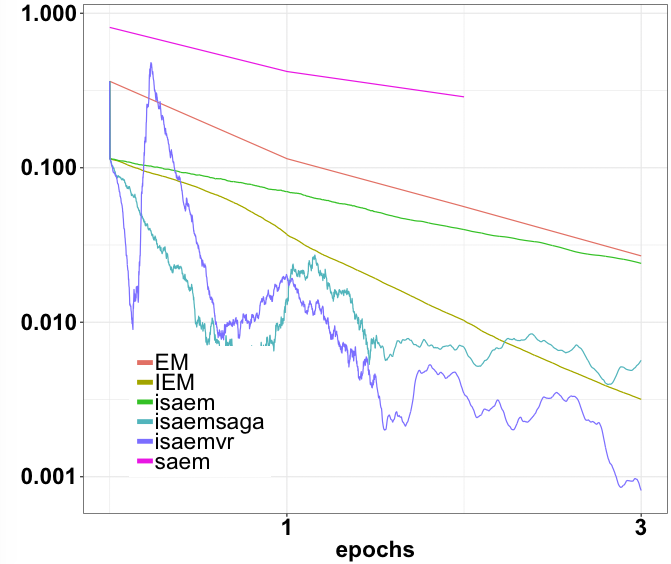
\includegraphics[width=.6\textwidth]{images/gmm}\vspace{-.3cm}
\caption{Performance of TTS methods for fitting a GMM. Precision ($| \mu^{(k)} - \mu^\star |^2$) as a function of the epoch elapsed.}
\label{fig:gmmplots}
\end{figure}

\end{frame}




\begin{frame}
\frametitle{Deformable Template for Image Analysis}
\begin{itemize}
\item  $(y_i, i \in \inter)$ images modelled as deformation of a template.
\item The model reads as follows:
$$y_{i}(s)=I\left(x_{s}-\Phi_{i}\left(x_{s}\right)\right)+\sigma \varepsilon_{i}(s)$$
where $s$ is the pixel index, $x_s$ its coordinate, $I$ the template and $\Phi_{i}$ the deformation.
\item The template model given $p_k$ landmarks on template and a fixed kernel:
\beq
I_{\xi}=\mathbf{K}_{\mathbf{p}} \xi, \quad \textrm{where} \quad \left(\mathbf{K}_{\mathbf{p}} \xi\right)(x)=\sum_{k=1}^{k_{p}} \mathbf{K}_{\mathbf{p}}\left(x, p_{k}\right) \xi(k)
\eeq
\item The deformation model given landmarks and a fixed kernel:
\beq
\Phi_{i}(x)=\left(\mathbf{K}_{\mathbf{g}} z_{i}\right)(x)=\sum_{k=1}^{k_{s}} \mathbf{K}_{\mathbf{g}}\left(x, g_{k}\right)\left(z_{i}^{(1)}(k), z_{i}^{(2)}(k)\right)
\eeq
\item We learn the parameters $\param = (\sigma, \xi, \Gamma)$ using the two-time-scale methods.

\end{itemize}
\end{frame}

\begin{frame}
\frametitle{Deformable Template for Image Analysis}
\begin{itemize}
\item USPS Digits Dataset
\item For a credit of epochs (running time maybe?), we generate images using the learnt model and see which one are similar to the template.

\begin{figure}[H]
\centering
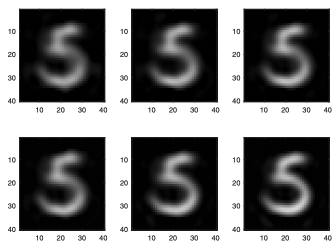
\includegraphics[width=.5\textwidth]{images/deformable2}\vspace{-.3cm}
\caption{Estimation of the template: first row : using SAEM (benchmark) ; second row : using new incremental method with minibatch size of $0.1$; columns correspond to 1, 2 and 3 epochs, respectively.}
\label{fig:gmmplots}
\end{figure}

\end{itemize}
\end{frame}

\begin{frame}
\frametitle{Deformable Template for Image Analysis}
\begin{itemize}

\item For a credit of number of images used in training.
\begin{figure}[H]
\centering
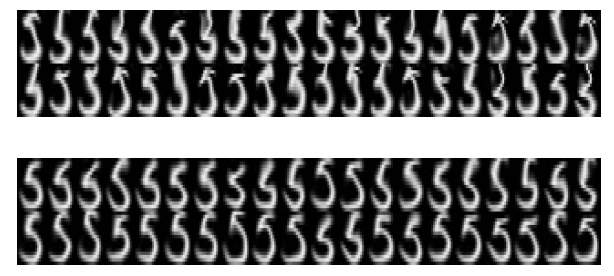
\includegraphics[width=.8\textwidth]{images/deformable}\vspace{-.3cm}
\caption{Synthetic images sampled from the model for digit 5 using the parameter estimates obtained with the batch version
on $20$ images (top) and with the mini-batch version with $1/5$th of the data with $100$ images.}
\label{fig:gmmplots}
\end{figure}

\end{itemize}
\end{frame}

\begin{frame}
\frametitle{ONGOING TASKS}
\begin{itemize}
\item Implement Deformable Template analysis on USPS digits
\item Proofs for Variance Reduction and Fast Incremental Two-Time-Scale methods
\item Finish writing
\end{itemize}
\end{frame}



\begin{frame}

\vfill
\begin{center}

{\huge Thank you! Questions?}\vspace{.3cm}

\end{center}

\vfill

\end{frame}
%
%\begin{frame}[allowframebreaks]
%
%\tiny
%
%\bibliographystyle{apalike}
%\bibliography{references}
%
%\end{frame}

\end{document}
